\chapter{2048と強化学習}
\label{chap:rl}
これまでに2048を対象とした強化学習の研究は数多くなされてきた. 
本章では強化学習の概要, および2048に対する強化学習の先行研究について記述する.

\section{強化学習の概要}
\label{sec:rl_general}
まず本節では2048との関係を踏まえつつ, 一般的な強化学習の概要について記述する.
なお本節の内容は全体に文献~\cite{Sutton1998}を参照して書かれた.

\subsection{マルコフ決定過程}
\label{subsec:mdp}
強化学習は与えられた環境において試行錯誤することを通して, 目標を達成するための戦略や意思決定を学習するための手法である.
学習や意思決定を行う主体はエージェントと呼ばれる.
エージェントは離散タイムステップに従って行動を選択し続け, 環境とやり取りを行う.

このような問題設定はマルコフ決定過程~(MDP)~というモデルによって定式化されている.
MDPは以下の$4$つの要素で構成される. 
\begin{itemize}
  \item 状態集合 $\mathcal{S}$
  \item 行動集合 $\mathcal{A}$
  \item 状態遷移関数$p:\mathcal{S} \times \mathcal{A} \times \mathcal{S} \rightarrow [0,1]$
  \item 報酬関数$r:\mathcal{S} \times \mathcal{A} \times \mathcal{S} \rightarrow \mathbb{R}$
\end{itemize}
エージェントはステップ$t$で状態$S_t \in \mathcal{S}$から行動$A_t \in \mathcal{A}$を選択する.
そして確率$p(S_{t+1}|S_t, A_t)$で次の状態$S_{t+1}$に遷移し, $R_{t+1} = r(S_t, A_t, S_{t+1})$を即時報酬として獲得する.
状態遷移関数と報酬関数は環境のダイナミクスと呼ばれることがある. 
図\ref{fig:mdp}にMDPの概念図を示す.
\begin{figure}[h]
  \centering
  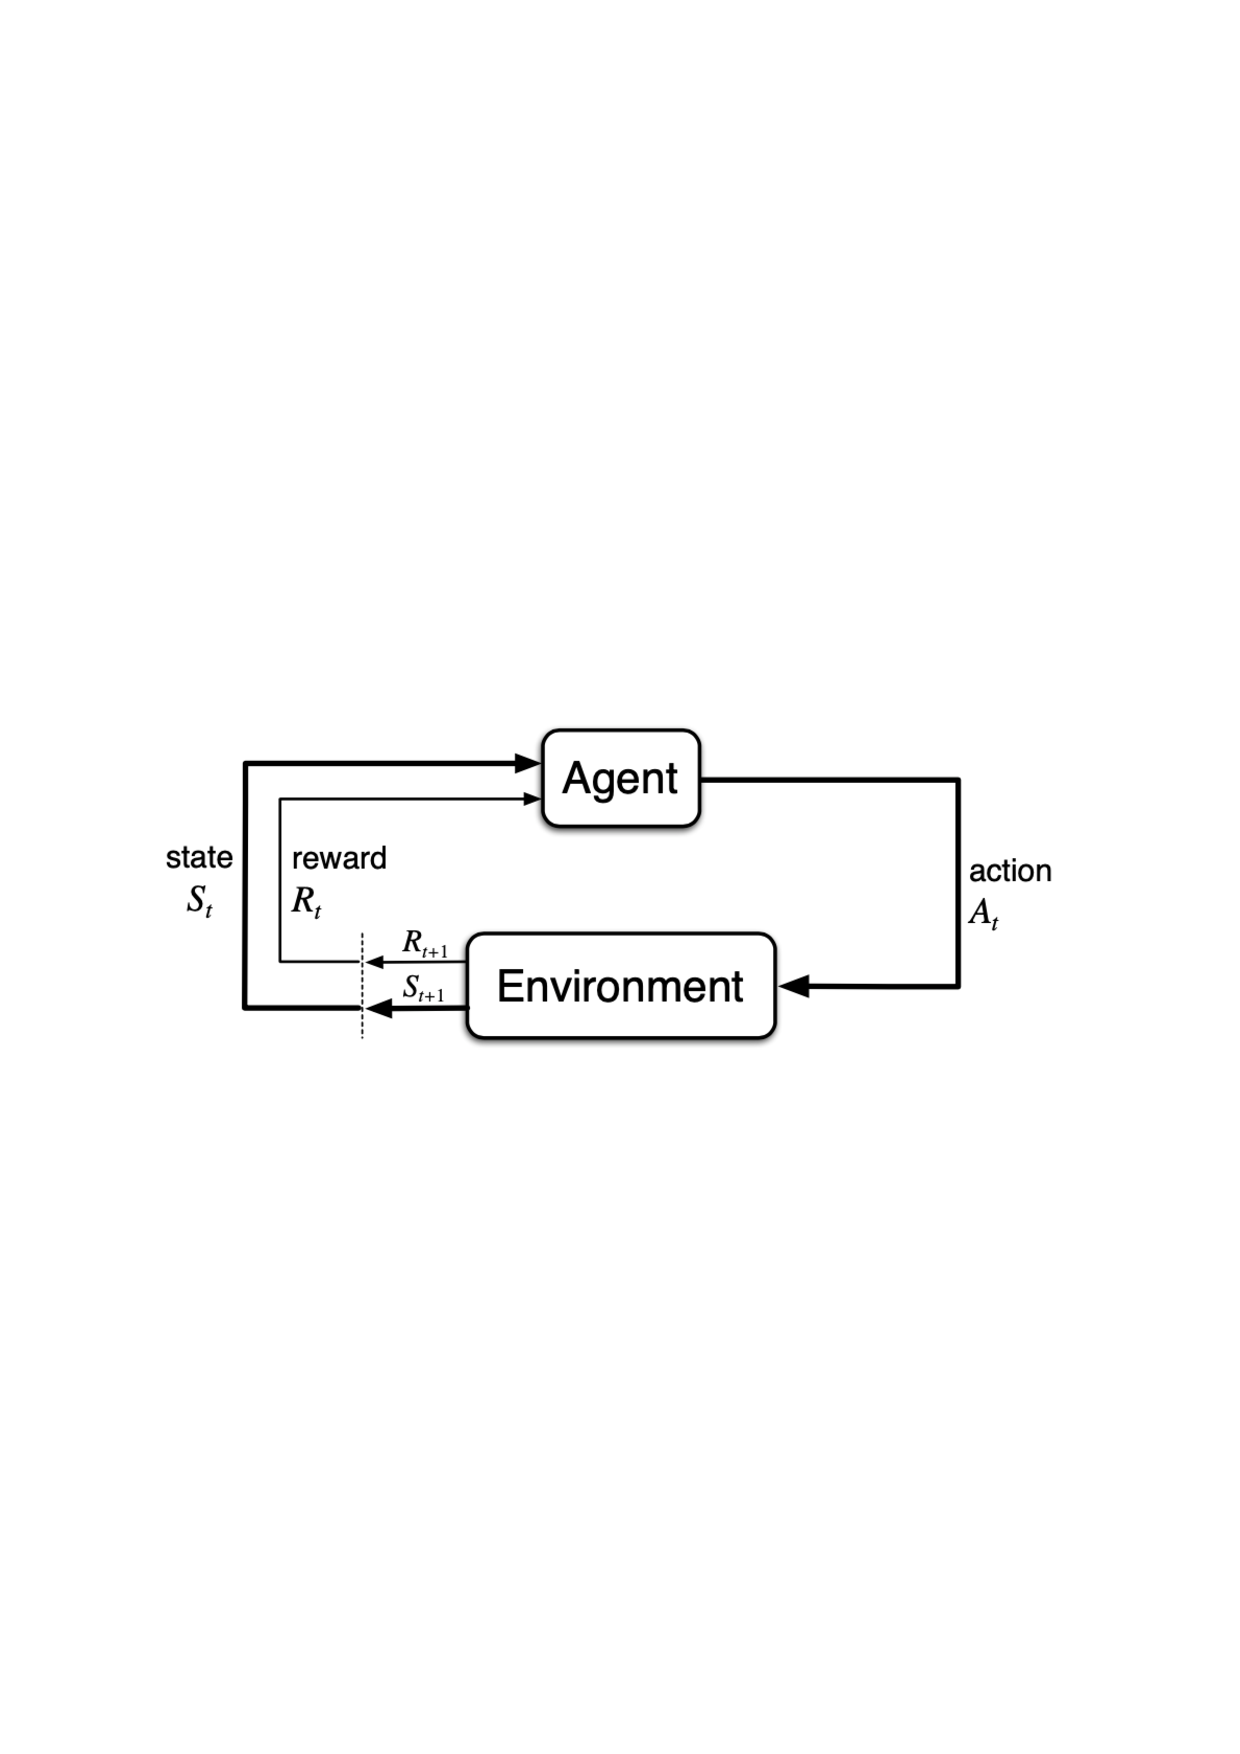
\includegraphics[width=\linewidth{}]{figures/MDP.pdf}
  \caption{MDPの模式図 (文献\cite{Sutton1998}より引用)}
  \label{fig:mdp}
\end{figure}

状態集合と行動集合が有限であるMDPを有限MDPと呼ぶ.
2048は有限MDPにそのまま当てはまるゲームである.
行動集合\textit{A}はプレイが選ぶ上下左右に対応し, 報酬はプレイヤが獲得する得点に直接対応する.

一般に強化学習で扱う問題には, エージェントと環境のやり取りが終わる終了状態が存在するepisodic taskと終了状態が存在しないcontinuing taskが存在する. 
episodic taskではエージェントと環境のやり取りを初期状態から終了状態までのエピソードと呼ばれる単位で分割することができる.
\ref{sec:property}節で説明したように2048は必ず終了するゲームであるため, 以降episodic taskでの定義を確認する. 

\subsection{方策と価値関数}
エージェントがある状態において行動を決定する際の戦略, すなわち確率分布$\pi:S \times A \rightarrow [0,1]$を方策と呼ぶ.
状態価値関数$v_{\pi}(s)$は状態$s$から方策$\pi$に従って行動を選択し続けた場合の累積報酬和の期待値であり, 次のように定義される.
\begin{align}
  v_{\pi}(s) \stackrel{\mathrm{def}}{=} \mathbb{E}_{\pi}\left[\sum_{k=0}^T \gamma^k R_{t+k+1}|S_t=s \right]
\end{align}
同様に状態$s$から行動$a$を選択し, その後方策$\pi$に従って行動を選択し続けた場合の累積報酬和の期待値である行動価値関数$q_{\pi}(s,a)$の定義は以下のようになる.
\begin{align}
  q_{\pi}(s,a) \stackrel{\mathrm{def}}{=} \mathbb{E}_{\pi}\left[\sum_{k=0}^T \gamma^k R_{t+k+1}|S_t=s, A_t=a \right]
\end{align}

強化学習の目標は多くの報酬を獲得できるような良い方策を見つけることである.
価値関数の定義より2つの方策$\pi$と$\pi'$があるとすると, すべての状態$s \in S$について$v_\pi(s) \geq v_{\pi'}(s)$が成り立つならば$\pi$は$\pi'$と等価か$\pi'$よりも良い方策だと言える.
ここで他のすべての方策と比べて等価であるか, それよりも良い方策が少なくとも$1$つ存在する.
これは最適方策$\pi_*$と呼ばれる方策である.
$\pi_*$に従うときの状態価値関数は最適状態価値関数と呼ばれ, $v_*$で表される.
同様に$\pi_*$に従うときの行動価値関数は最適行動価値関数と呼ばれ, $q_*$で表される.
それぞれの具体的な定義を式~\ref{eq:v_opt}, \ref{eq:q_opt}に示す.
\begin{align}
  \label{eq:v_opt}
  v_*(s) &= \max_\pi v_{\pi}(s) \quad \text{for all } s \in S \\
  \label{eq:q_opt}
  q_*(s,a) &= \max_\pi q_{\pi}(s, a) \quad \text{for all } s \in S \text{ and } a \in A(s)
\end{align}
このとき$v_*(s) = \max_{a \in A(s)} q_*(s, a)$であるから, 以下の式が導かれる~(図~\ref{fig:backup}を参照)~.
\begin{align}
  v_*(s) &= \max_{a \in A(s)} q_*(s, a) \\
  \label{eq:bellman_v_opt}
               &= \max_{a \in A(s)} \mathbb{E}[R_{t+1} + \gamma v_*(S_{t+1}) | S_t=s, A_t=a] \\
  q_*(s, a) &= \mathbb{E}[R_{t+1} + \gamma v_*(S_{t+1}) | S_t=s, A_t=a] \\
  \label{eq:bellman_q_opt}
                  &= \mathbb{E}[R_{t+1} + \gamma \max_{a'} q_*(S_{t+1}, a') | S_t=s, A_t=a]
\end{align}
式~\ref{eq:bellman_v_opt}, \ref{eq:bellman_q_opt}はベルマン最適方程式と呼ばれる.
\begin{figure}[h]
  \centering
  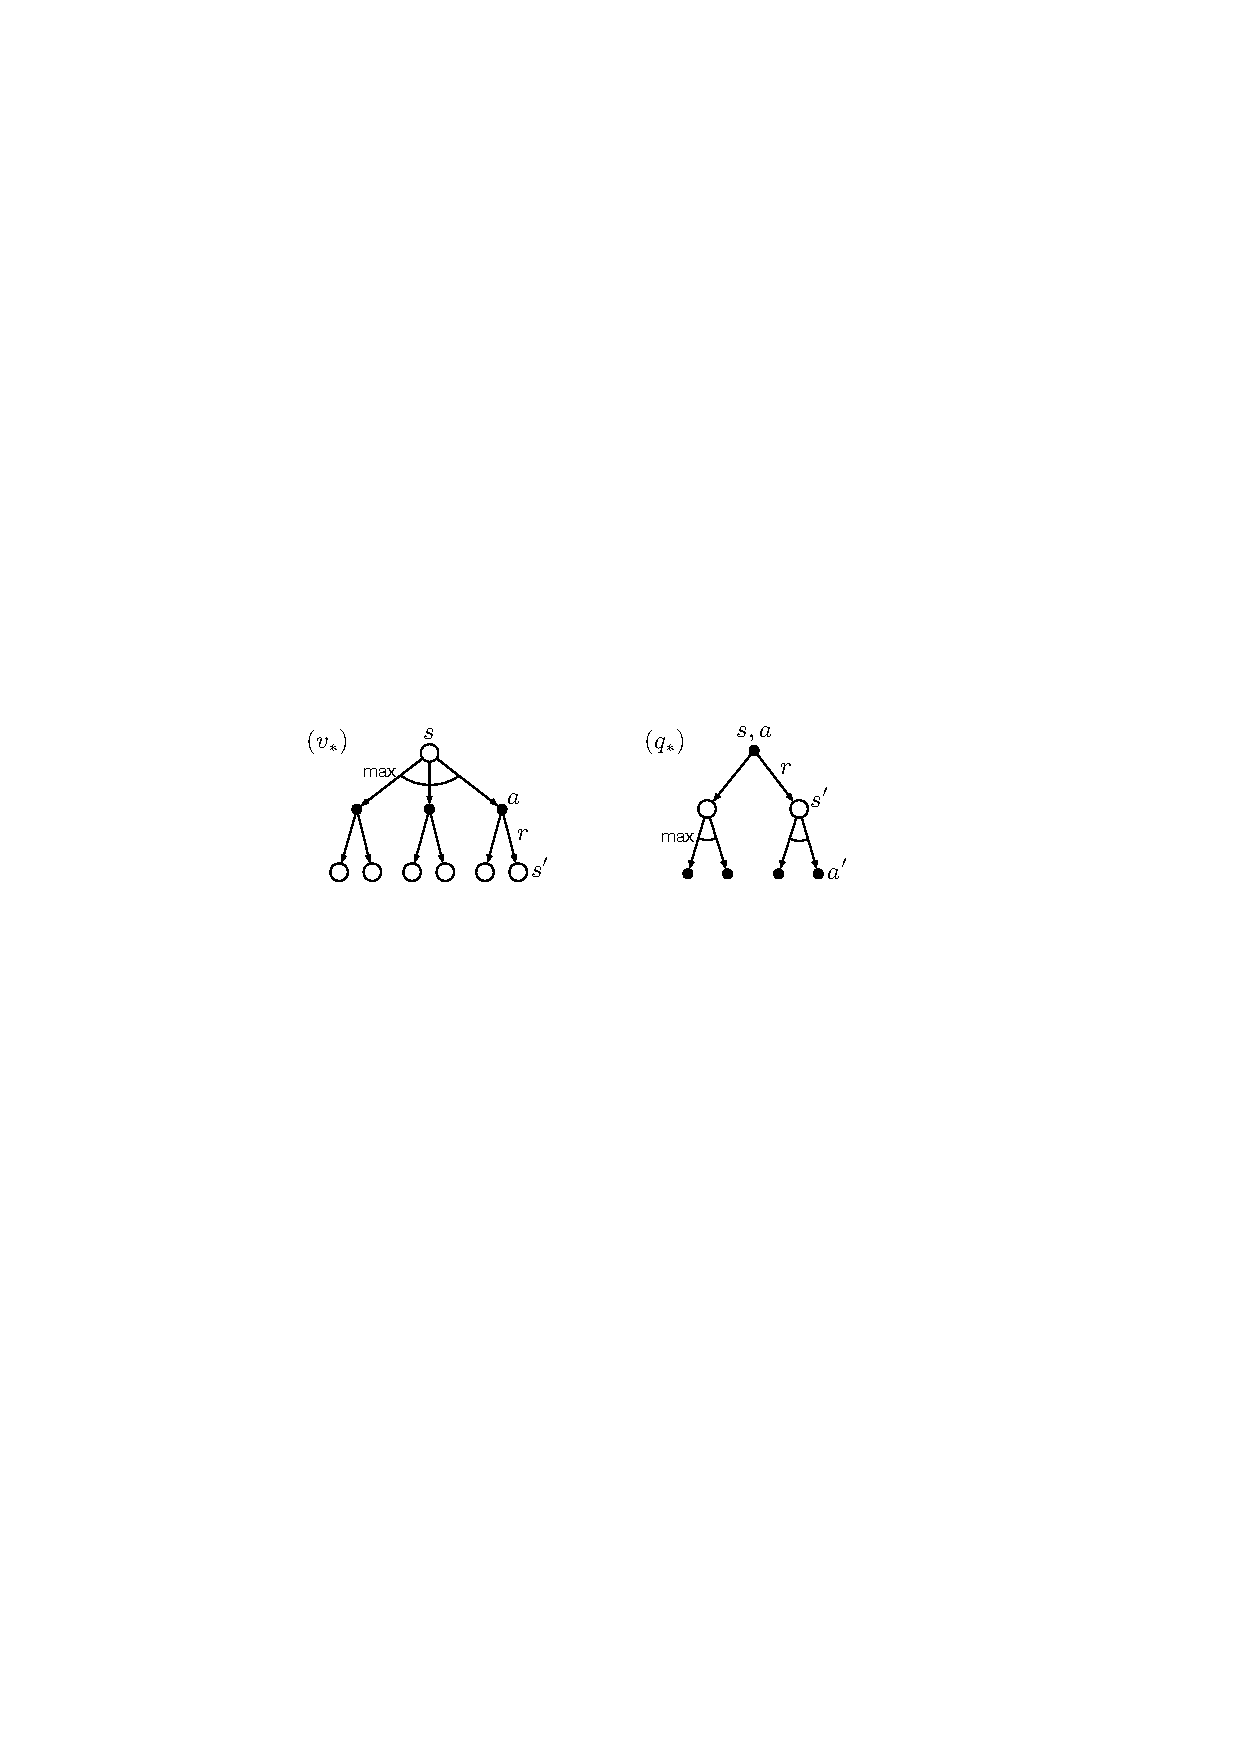
\includegraphics[width=\linewidth{}]{figures/backup.pdf}
  \caption{最適価値関数のバックアップ図 (文献\cite{Sutton1998}より引用)}
  \label{fig:backup}
\end{figure}

\subsection{価値ベースな手法}
状態$s$における最適方策に従った具体的な行動は$\argmax \mathbb{E}[R_{t+1} + \gamma v_*(S_{t+1}) | S_t=s, A_t=a]$と, $1$ステップ先の状態を探索してそれらの最適状態価値関数を参照することで計算できる.
最適行動価値関数が参照できれば, $1$ステップ先の状態を探索する必要すらなく, 単に$\argmax q_*(s, a)$を選択すればよい.
最適方策を得るために価値関数を学習する手法は価値ベースな手法と呼ばれる.

Q学習は最も基本的な価値ベースな手法の$1$つで, 最適行動価値関数$q_*$の推定値$Q$を得られた経験から学習する.
状態$S_t$から行動$A_t$を選択し, 報酬$R_{t+1}$を獲得して次の状態$S_{t+1}$に遷移したとする.
このときQ学習は以下の更新式~\ref{eq:q_learning}に従って$Q(S_t, A_t)$を更新する.
\begin{align}
  \label{eq:q_learning}
  Q(S_t, A_t) \leftarrow Q(S_t, A_t) + \alpha [R_{t+1} + \gamma \max_a Q(S_{t+1}, a) - Q(S_t, A_t)] 
\end{align}
式~\ref{eq:q_learning}は現在の推定値$Q(S_t, A_t)$を, ベルマン最適方程式~\ref{eq:bellman_q_opt}の右辺の推定値である$R_{t+1} + \gamma \max_a Q(S_{t+1}, a)$に近づけていると解釈できる.
任意の$(s, a) \in \mathcal{S} \times \mathcal{A}$について$Q(s,a)$が更新され続けるという条件の下で, Q学習は収束が保証されている.

状態集合や行動集合が大きい場合や有限でない場合には, テーブル形式でQ値を保持することができないため何らかの関数近似を行う必要がある.
近年では深層学習~\cite{DeepLearning}の研究の発展により, 関数近似の方法としてニューラルネットワークが用いられることが多い.
価値関数や方策をニューラルネットワークで近似する手法は, まとめて深層強化学習と呼ばれる.
Q値をニューラルネットワークで近似する, Deep Q Network~(DQN)~\cite{DQN}は深層強化学習の先駆けとして有名な手法である. 
DQNの発表以降, 様々な工夫が提案され続けている.
詳細は文献~\cite{deepRL}の$4$節などを参照されたい.

\subsection{方策ベースな手法}
方策を直接パラメタライズされた関数で近似し, 目的関数との誤差を最小化するようにパラメータを学習する手法を全般に方策ベースな手法と呼ぶ.
方策ベースな手法においても価値関数の学習を行うことはあるが, あくまで良い方策のパラメータを学習するために必要とするもので, 直接的な行動の選択には関与しない.

方策のパラメータを$\theta$として目的関数を$J(\theta)$とする.
$J(\theta)=v_{\theta}(s_0)$
方策ベースな深層強化学習手法としては, Schulmanらが提案したProximal Policy Optimization~(PPO)~\cite{PPO}が有名である.

\section{AlphaZeroとMuZero}
Silverらが提案したAlphaZero~\cite{AlphaZero}は, 囲碁やチェスなどの二人零和完全確定情報ゲームを対象とした有力な深層強化学習手法である.
AlphaZeroは盤面の特徴量を入力として, その盤面における方策と価値を出力するニューラルネットワークを, 自己対戦を通して得たデータから学習する.
自己対戦において, AlphaZeroはモンテカルロ木探索~(MCTS)~というアルゴリズムを使用して指し手を選択する.

\subsection{モンテカルロ木探索}
ここではAlphaZeroが使用したモンテカルロ木探索~(MCTS)~について説明する.
MCTSは探索で発見した各状態~(囲碁や将棋では盤面)~に対応するノードから成る探索木を構築する.
探索木中のそれぞれの状態と行動の対~$(s,a)$~について, ${N(s,a), W(s,a), Q(s,a), P(s,a)}$という$4$つの統計量を管理する.
\begin{itemize}
  \item $N(s,a) \cdots$探索中に$s$から$a$を選択した回数
  \item $W(s,a) \cdots$最適行動価値$q_*(s,a)$の推定値の累計
  \item $Q(s,a) \cdots$最適行動価値$q_*(s,a)$の推定値の平均~($W(s,a) / N(s,a)$)
  \item $P(s,a) \cdots$ニューラルネットワークが評価する$s$から$a$を選択する確率
\end{itemize}
探索木は最初, 現在の状態に対応するノードである根ノードのみから成る.
MCTSは選択, 評価, 逆伝播, 展開の$4$つのステップを繰り返すことで, 探索木を大きくする.
この$4$つのステップはまとめてシミュレーションと呼ばれる.
すなわちシミュレーションを繰り返すことで深い探索を行い, 良い行動を選択することができる.
以下ではそれぞれのステップについて説明する.
\subsubsection*{選択~(図~\ref{fig:selection})}
現在のゲーム木の根ノード$s_0$から有望な行動を選択し, 葉ノード$s_L$に至るまで辿り続ける.
具体的にはノード$s_t$において,以下の式~\ref{eq:puct}で表される$a_t$を選択する.
\begin{align}
  a_t = \argmax_a(Q(s_t,a) + C(s_t)P(s_t,a)\sqrt{N(s_t)}/(1 + N(s_t,a)))
  \label{eq:puct}
\end{align}
ただし$C(s_t)$は探索率, $N(s_t)$はノード$s_t$の訪問回数を表す.
これは現段階での価値の推定値$Q(s_t,a)$と探索項$C(s_t)P(s_t,a)\sqrt{N(s_t)}/(1 + N(s_t,a))$を合計したものである.
$N(s_t,a)$が小さい行動ほど探索項は大きな値を示す.

\subsubsection*{評価~(図~\ref{fig:evaluate})}
選択のステップの葉ノード$s_L$をニューラルネットワーク$f_\theta$により評価する.
$f_\theta$が評価した$s_L$における方策を$\pi(\cdot|s_L)$, $s_L$の価値を$v_L$とする.

\subsubsection*{逆伝播~(図~\ref{fig:backpropagate})}
$s_L$から選択可能なそれぞれの行動$a$について, $N(s_L, a)=0, W(s_L, a)=0, Q(s_L, a)=0, P(s_L, a)=\pi(a|s_L)$と初期化する.
さらに$s_0$から$s_L$に至る各エッジ$(s_t,a_t)$について, 以下のように各統計量の値を更新する.
\begin{align*}
  N(s_t, a_t) &= N(s_t, a_t)+1 \\
  W(s_t, a_t) &= W(s_t, a_t) + v_L \\
  Q(s_t, a_t) &= \frac{W(s_t,a_t)}{N(s_t,a_t)}
\end{align*}

\subsubsection*{展開~(図~\ref{fig:expand})}
$s_L$から遷移しうる次の状態を新たなノードとして探索木に追加する.

\subsubsection*{行動の決定方法}
一定回数のシミュレーションを行った後に, 実際に選ぶ行動を決定する.
根ノード$s_0$から選択可能な各行動$a$について, $N(s_0, a)^{1/\tau}$に比例した確率で行動を選択する.
$\tau$は温度パラメータと呼ばれ, $0$に近づくほど訪問回数に関して貪欲な選択をするようになる.
多様な学習データを集めるために学習の序盤では$\tau$を大きく設定し, 学習が進むについて$0$に近づける.

\begin{figure}
  \begin{subfigure}[T]{0.4\columnwidth}
    \centering
    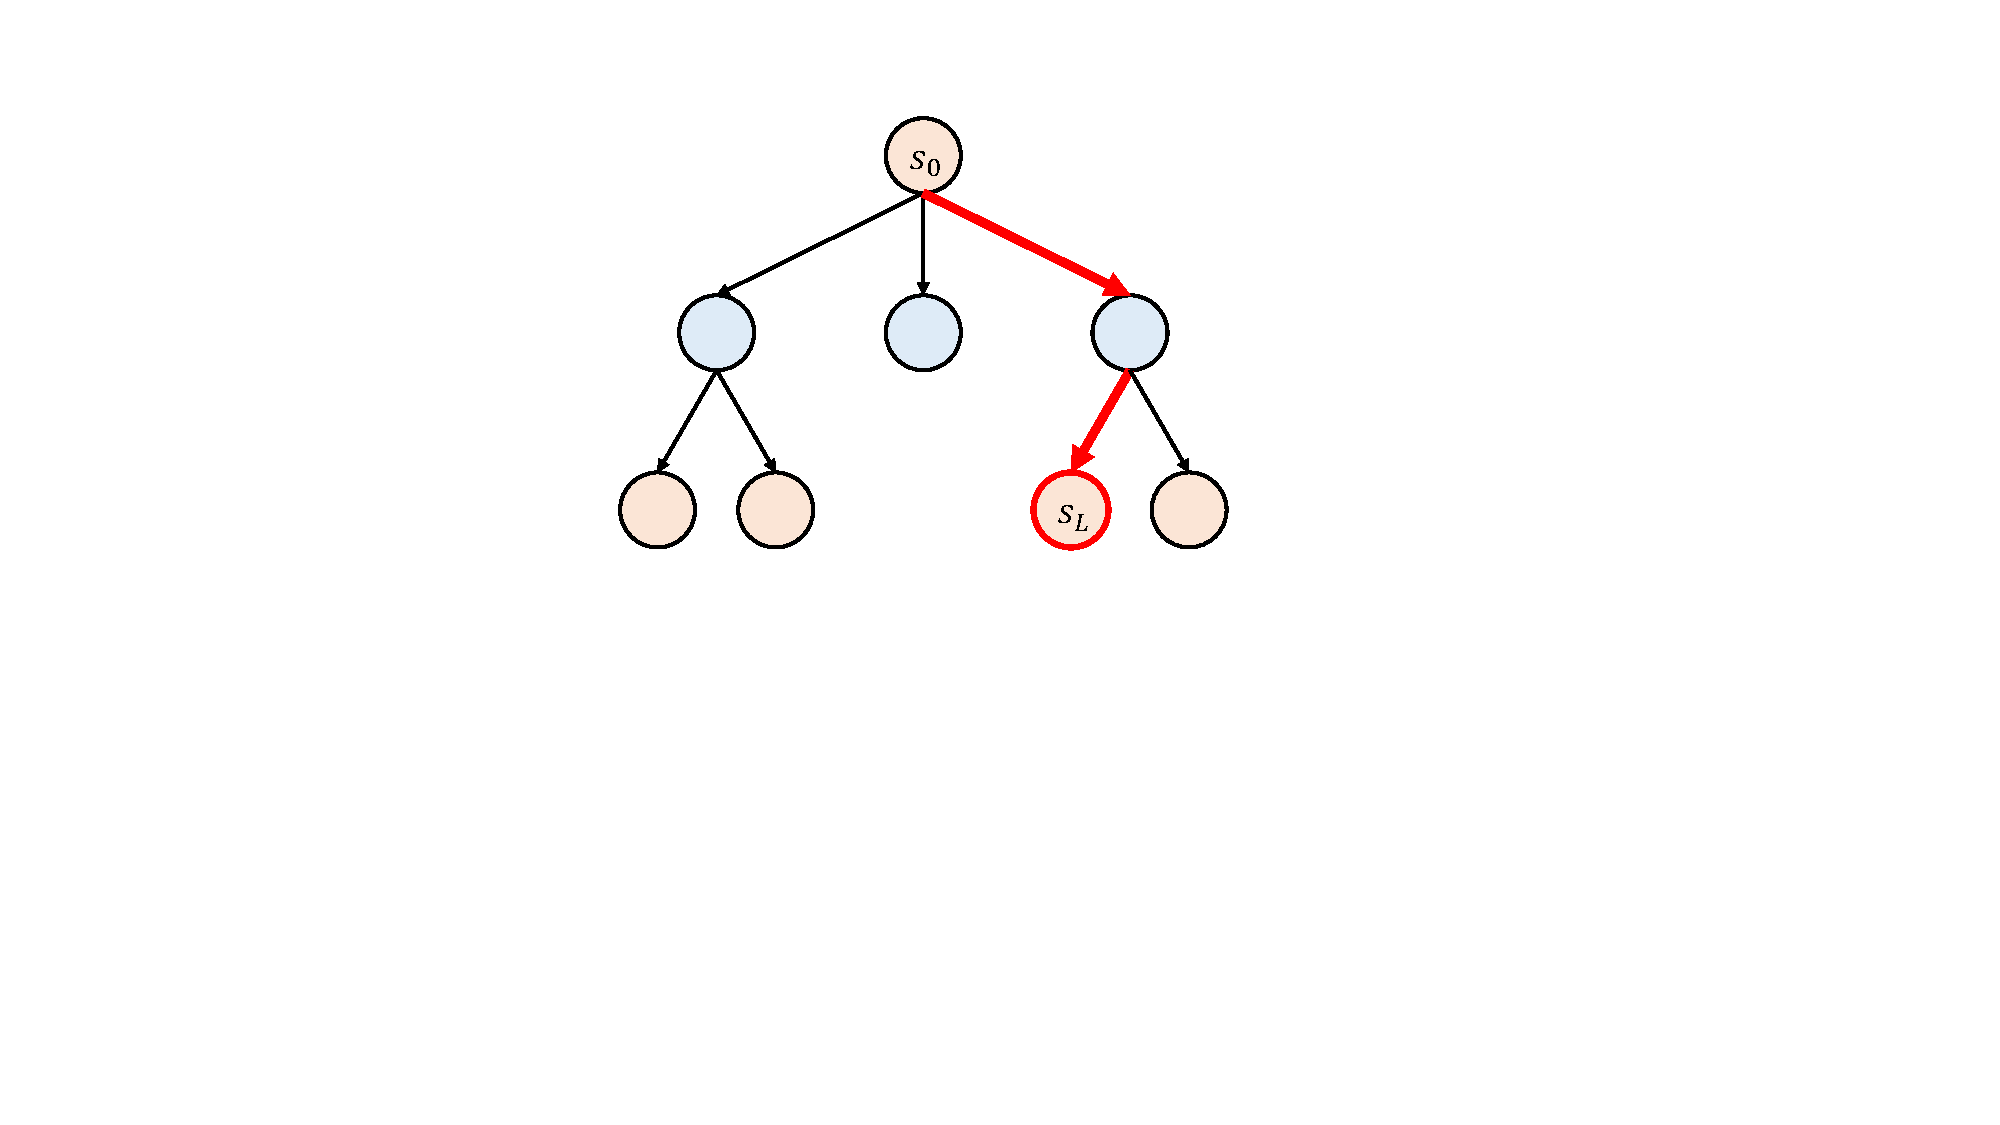
\includegraphics[width=\columnwidth]{figures/selection_.pdf}
    \caption{選択}
    \label{fig:selection}
  \end{subfigure}
  \begin{subfigure}[T]{0.4\columnwidth}
    \centering
    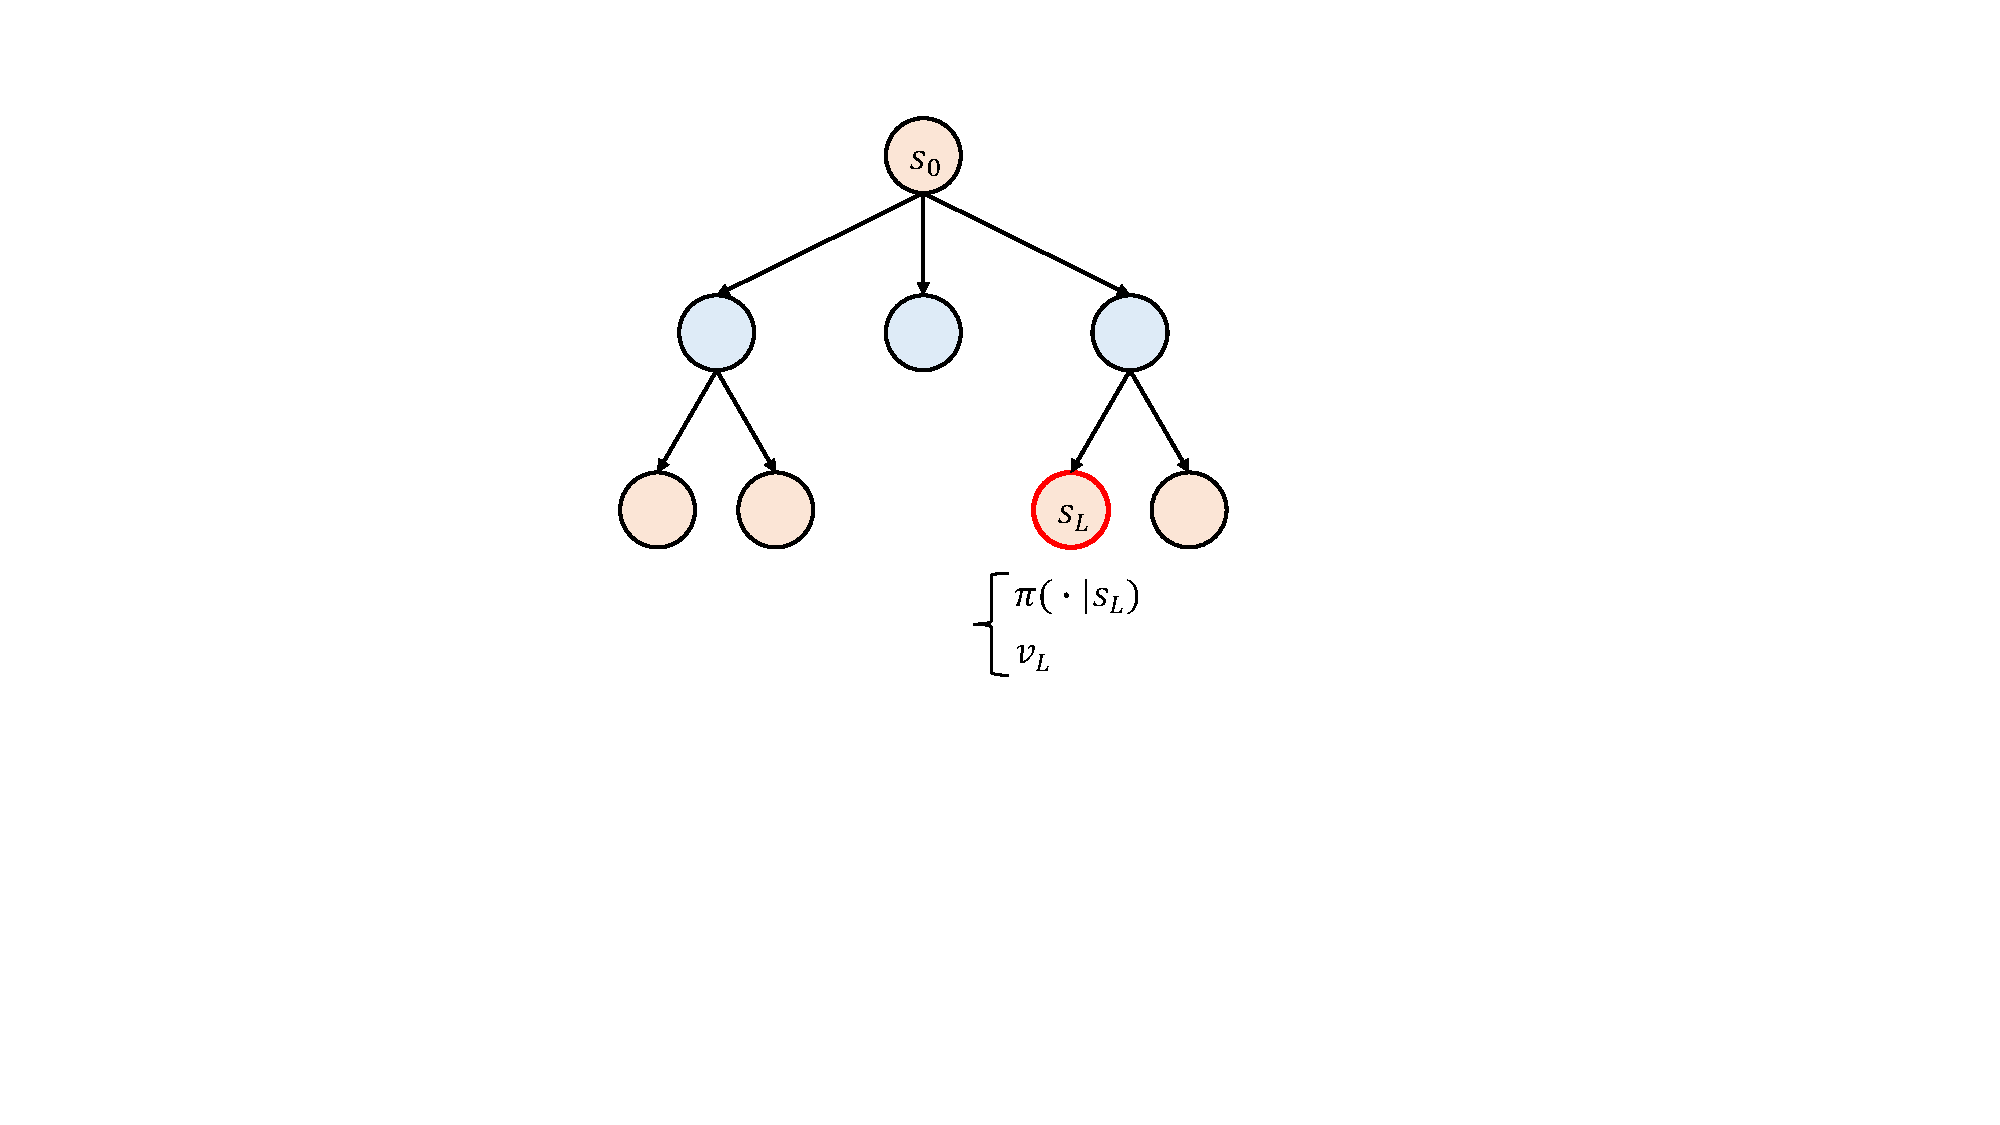
\includegraphics[width=\columnwidth]{figures/evaluate_.pdf}
    \caption{評価}
    \label{fig:evaluate}
  \end{subfigure}
  \begin{subfigure}[T]{0.4\columnwidth}
    \centering
    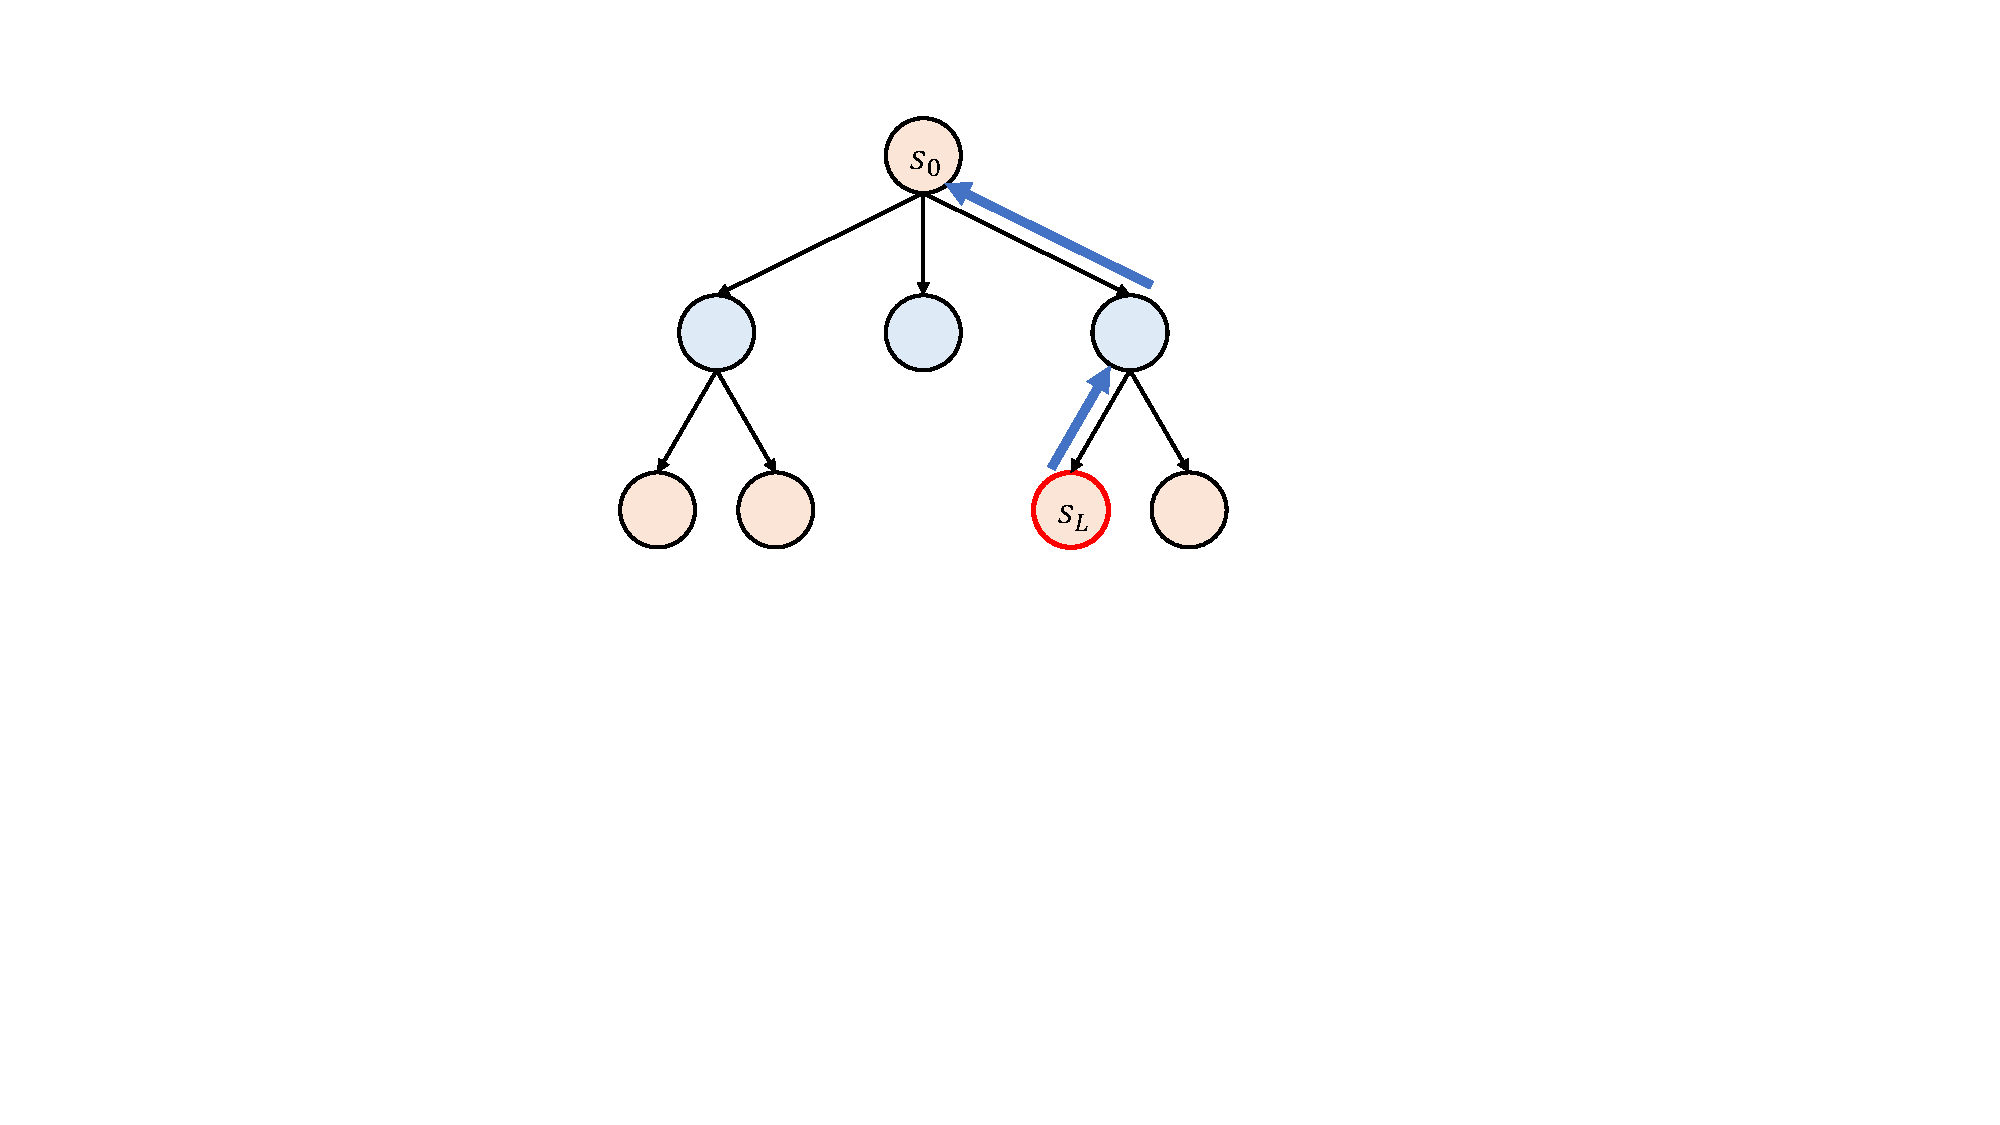
\includegraphics[width=\columnwidth]{figures/backpropagate_.pdf}
    \caption{逆伝播}
    \label{fig:backpropagate}
  \end{subfigure}
  \hspace{3cm}
  \begin{subfigure}[T]{0.4\columnwidth}
    \centering
    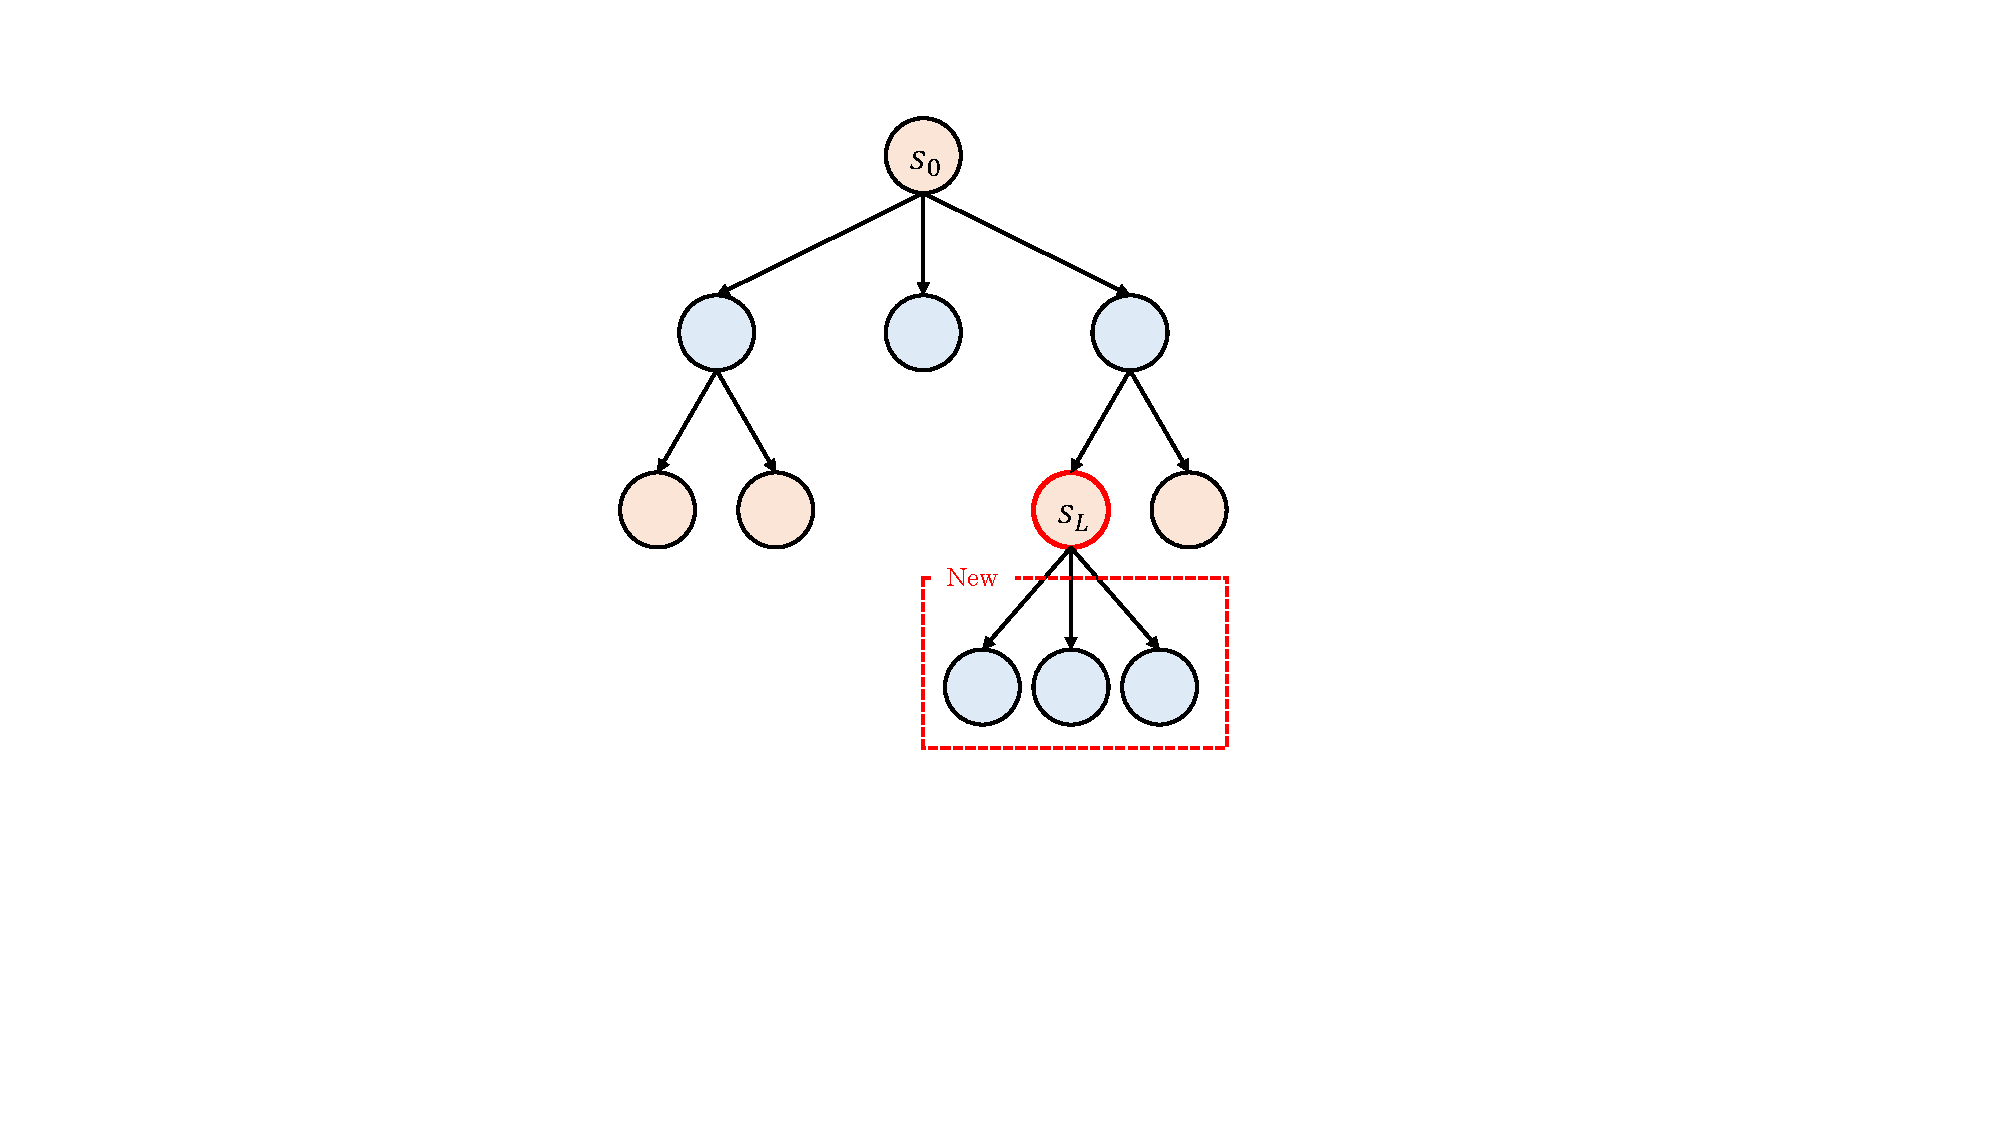
\includegraphics[width=\columnwidth]{figures/expand_.pdf}
    \caption{展開}
    \label{fig:expand}
  \end{subfigure}
  \caption{MCTSの各ステップ~(オレンジ色のノードは自分の手番, 青色のノードは相手の手番)}
  \label{fig:mcts}
\end{figure}

\subsection{自己対戦とニューラルネットワークの学習}
AlphaZeroは人間の棋譜ではなく, 自己対戦によって得た学習データを使ってニューラルネットワークを訓練する.
自己対戦は, 
各訪問回数を正規化した$\pmb{\pi}$
すなわち式~\ref{eq:az_loss}で表される誤差関数$l$を最小化するようにパラメータを更新する.
\begin{align}
\label{eq:az_loss}
l = (z-v)^2 - \pmb{\pi}^{\mathrm{T}} \log \mathbf{p}
\end{align}

\subsection{AlphaZeroの評価とMuZero}
\label{subsec: muzero}
囲碁, 将棋, チェスにおいて当時の有力なプログラムを上回る強さを示して注目を集めた.
AlphaZeroが行うMCTSは, ゲームのルールや環境のダイナミクスが既知であることを前提としている.
すなわち現在の状態$s_t$から行動$a_t$を選択した後の状態$s_{t+1}$を, $s_t$のみ観測可能な状況から知ることができる必要がある.
そのためAlphaZeroは複雑なダイナミクスを持つAtariなどのゲームには適用することが難しい.
Schrittwieserらが提案したMuZero~\cite{MuZero}は, ニューラルネットワークで環境のダイナミクスをモデル化し, 学習することを提案した.

\section{2048への強化学習の応用}
\label{sec:rlto2048}
\ref{sec:rl_general}節では強化学習一般の概要について説明した.
これを踏まえて本節では, 2048を対象とした強化学習研究の先行研究について概説する.

\subsection{TD afterstate学習}
\label{subsec: td_afterstate}
Szubertら~\cite{Szubert}はTD afterstate学習と呼ばれる価値ベースの強化学習手法を提案した.
2048はゲームの性質上, 状態$s$から行動$a$をとって獲得する得点$r(s,a)$と遷移するafterstate $s'$は決定的である.
よってafterstate $s'$の最適価値を$v_*'(s')$と表すと, 行動価値$q_*(s,a)$は$q_*(s,a) = r(s,a) + v_*'(s')$と分解できる.
そこでTD afterstate学習は, Q値ではなくafterstateの価値$v_*'$の推定値$V'$を式~\ref{eq:td_afterstate}に従って更新する.
\begin{align}
  \label{eq:td_afterstate}
  V'(S_{t}^{'}) \leftarrow  V'(S_{t}^{'}) + \alpha [R_{t+1} + V'(S_{t+1}^{'}) - V'(S_{t}^{'})]
\end{align}
式~\ref{eq:td_afterstate}はQ学習の更新式~\ref{eq:q_learning}において, $Q(S_t, A_t) = R(S_t, A_t) + V'(S_{t}^{'})$として書き直したものと見ることができる.

SzubertらはN-tupleネットワークというヒューリスティックな盤面評価関数を用いて$V'$を表現し, $2048$のタイルを$98$\%の確率で到達させることに成功した.
Jaskowski~\cite{DBLP:journals/corr/Jaskowski16}はこれに様々な工夫を加えた学習方法を提案し, 最終的にexpectimax探索を$1$手$1$秒の制限で行うことで平均$609,104$点を獲得するプレイヤを開発した.
松崎~\cite{KiminoriMatsuzaki2021}はニューラルネットワークによって表現した$V'$を学習させ, $3$-ply expectimax探索を行うことで平均$406,927$点を達成した.

Szubertらは文献~\cite{Szubert}でN-tupleネットワークを用いたQ学習の実験も行ったが, TD afterstate学習の性能を大きく下回る結果になったことを報告している.
TD afterstate学習は観測している状態$s$からafterstate $s'$への遷移までをシミュレートする, いわば$0.5$手読みの探索を行っているため, $0$手読みのQ学習と比べて学習しやすいと考えられる.

\subsection{Afterstate PPO}
価値ベースな手法であるTD afterstate学習が一方で方策ベースな強化学習手法で2048を
山下ら~\cite{afterstate_ppo}は

\subsection{Stochastic MuZero}
Antonoglouらが提案したStochastic MuZero~\cite{StochasticMuZero}は~\ref{subsec: muzero}節で述べたMuZeroを, 確率的な環境にも対応できるように拡張した手法である.
Stochastic MuZeroは確率的ゲームである2048とバックギャモンでMuZeroを大きく上回るパフォーマンスを発揮した.
さらにランダム性のない囲碁においてもMuZeroと同等のレーティングを達成し, 対象とするドメインが幅広いことを示した.

2048においては, \ref{subsec: td_afterstate}節で述べたTD afterstate学習の先行研究~\cite{DBLP:journals/corr/Jaskowski16}と比較して, 一切のドメイン知識を必要とせず, より優れたパフォーマンスを出したことが強調された.
一方で, 論文内で示されたStochastic MuZeroの最終的な平均スコアは約$50$万点で, expectimax探索を行うことで平均$609,104$点を達成した文献~\cite{DBLP:journals/corr/Jaskowski16}の結果を明確に上回るとはいえない.
以下では具体的に2048へ適用することを想定した手法の説明を行う.

Stochastic MuZeroは以下の$5$つのニューラルネットワークを学習する.
\begin{itemize}
  \item \textit{Representation}ネットワーク $h$
  \item \textit{Prediction}ネットワーク $f$
  \item \textit{Afterstate Dynamics}ネットワーク $\phi$
  \item \textit{Afterstate Prediction}ネットワーク $\psi$
  \item \textit{Dynamics}ネットワーク $g$
\end{itemize}

まずStochastic MuZeroは\textit{decisionノード}と\textit{chanceノード}という2種類のノードから成る探索木を用いてMCTSを行う.
decisionノードはプレイやが行動を選択する状態に対応し, chanceノードはafterstateに対応する.
decisionノードからchanceノードへの遷移は決定的で, chanceノード
これは$1$回の確率的な遷移を, 決定的な部分~(decisionノード)~と確率的な部分~(chanceノード)~に分けているといえる.
2048においてdecisionノードはプレイやが行動を選択する状態に対応し, chanceノードはafterstateに対応している.

\begin{table}[t]
  \centering
  \begin{tabular}{clll}
   \hline
   手法 & 対象ドメイン & 測定方法 & 測定結果 \\
   \hline \hline
   AlphaZero & 二人零和有限完全確定情報ゲーム & 二人が離れてランプの光を見る & (音速10倍以上) \\
   MuZero & 二人零和有限完全確定情報ゲーム + Atari & 木星の衛星の観測から & 2 \\
   Stochastic MuZero & Bradley & 星の収差から & 3.01 \\
   \hline
  \end{tabular}
\end{table}

\subsection{先行研究の考察}